
%% bare_jrnl.tex
%% V1.3
%% 2007/01/11
%% by Michael Shell
%% see http://www.michaelshell.org/
%% for current contact information.
%%
%% This is a skeleton file demonstrating the use of IEEEtran.cls
%% (requires IEEEtran.cls version 1.7 or later) with an IEEE journal paper.
%%
%% Support sites:
%% http://www.michaelshell.org/tex/ieeetran/
%% http://www.ctan.org/tex-archive/macros/latex/contrib/IEEEtran/
%% and
%% http://www.ieee.org/



% *** Authors should verify (and, if needed, correct) their LaTeX system  ***
% *** with the testflow diagnostic prior to trusting their LaTeX platform ***
% *** with production work. IEEE's font choices can trigger bugs that do  ***
% *** not appear when using other class files.                            ***
% The testflow support page is at:
% http://www.michaelshell.org/tex/testflow/


%%*************************************************************************
%% Legal Notice:
%% This code is offered as-is without any warranty either expressed or
%% implied; without even the implied warranty of MERCHANTABILITY or
%% FITNESS FOR A PARTICULAR PURPOSE! 
%% User assumes all risk.
%% In no event shall IEEE or any contributor to this code be liable for
%% any damages or losses, including, but not limited to, incidental,
%% consequential, or any other damages, resulting from the use or misuse
%% of any information contained here.
%%
%% All comments are the opinions of their respective authors and are not
%% necessarily endorsed by the IEEE.
%%
%% This work is distributed under the LaTeX Project Public License (LPPL)
%% ( http://www.latex-project.org/ ) version 1.3, and may be freely used,
%% distributed and modified. A copy of the LPPL, version 1.3, is included
%% in the base LaTeX documentation of all distributions of LaTeX released
%% 2003/12/01 or later.
%% Retain all contribution notices and credits.
%% ** Modified files should be clearly indicated as such, including  **
%% ** renaming them and changing author support contact information. **
%%
%% File list of work: IEEEtran.cls, IEEEtran_HOWTO.pdf, bare_adv.tex,
%%                    bare_conf.tex, bare_jrnl.tex, bare_jrnl_compsoc.tex
%%*************************************************************************

% Note that the a4paper option is mainly intended so that authors in
% countries using A4 can easily print to A4 and see how their papers will
% look in print - the typesetting of the document will not typically be
% affected with changes in paper size (but the bottom and side margins will).
% Use the testflow package mentioned above to verify correct handling of
% both paper sizes by the user's LaTeX system.
%
% Also note that the "draftcls" or "draftclsnofoot", not "draft", option
% should be used if it is desired that the figures are to be displayed in
% draft mode.
%
\documentclass[journal]{IEEEtran}
%
% If IEEEtran.cls has not been installed into the LaTeX system files,
% manually specify the path to it like:
% \documentclass[journal]{../sty/IEEEtran}





% Some very useful LaTeX packages include:
% (uncomment the ones you want to load)


% *** MISC UTILITY PACKAGES ***
%
%\usepackage{ifpdf}
% Heiko Oberdiek's ifpdf.sty is very useful if you need conditional
% compilation based on whether the output is pdf or dvi.
% usage:
% \ifpdf
%   % pdf code
% \else
%   % dvi code
% \fi
% The latest version of ifpdf.sty can be obtained from:
% http://www.ctan.org/tex-archive/macros/latex/contrib/oberdiek/
% Also, note that IEEEtran.cls V1.7 and later provides a builtin
% \ifCLASSINFOpdf conditional that works the same way.
% When switching from latex to pdflatex and vice-versa, the compiler may
% have to be run twice to clear warning/error messages.






% *** CITATION PACKAGES ***
%
\usepackage{cite}
% cite.sty was written by Donald Arseneau
% V1.6 and later of IEEEtran pre-defines the format of the cite.sty package
% \cite{} output to follow that of IEEE. Loading the cite package will
% result in citation numbers being automatically sorted and properly
% "compressed/ranged". e.g., [1], [9], [2], [7], [5], [6] without using
% cite.sty will become [1], [2], [5]--[7], [9] using cite.sty. cite.sty's
% \cite will automatically add leading space, if needed. Use cite.sty's
% noadjust option (cite.sty V3.8 and later) if you want to turn this off.
% cite.sty is already installed on most LaTeX systems. Be sure and use
% version 4.0 (2003-05-27) and later if using hyperref.sty. cite.sty does
% not currently provide for hyperlinked citations.
% The latest version can be obtained at:
% http://www.ctan.org/tex-archive/macros/latex/contrib/cite/
% The documentation is contained in the cite.sty file itself.






% *** GRAPHICS RELATED PACKAGES ***
%
\ifCLASSINFOpdf
   \usepackage[pdftex]{graphicx}
  % declare the path(s) where your graphic files are
  % \graphicspath{{../pdf/}{../jpeg/}}
  % and their extensions so you won't have to specify these with
  % every instance of \includegraphics
  % \DeclareGraphicsExtensions{.pdf,.jpeg,.png}
\else
  % or other class option (dvipsone, dvipdf, if not using dvips). graphicx
  % will default to the driver specified in the system graphics.cfg if no
  % driver is specified.
  % \usepackage[dvips]{graphicx}
  % declare the path(s) where your graphic files are
  % \graphicspath{{../eps/}}
  % and their extensions so you won't have to specify these with
  % every instance of \includegraphics
  % \DeclareGraphicsExtensions{.eps}
\fi
% graphicx was written by David Carlisle and Sebastian Rahtz. It is
% required if you want graphics, photos, etc. graphicx.sty is already
% installed on most LaTeX systems. The latest version and documentation can
% be obtained at: 
% http://www.ctan.org/tex-archive/macros/latex/required/graphics/
% Another good source of documentation is "Using Imported Graphics in
% LaTeX2e" by Keith Reckdahl which can be found as epslatex.ps or
% epslatex.pdf at: http://www.ctan.org/tex-archive/info/
%
% latex, and pdflatex in dvi mode, support graphics in encapsulated
% postscript (.eps) format. pdflatex in pdf mode supports graphics
% in .pdf, .jpeg, .png and .mps (metapost) formats. Users should ensure
% that all non-photo figures use a vector format (.eps, .pdf, .mps) and
% not a bitmapped formats (.jpeg, .png). IEEE frowns on bitmapped formats
% which can result in "jaggedy"/blurry rendering of lines and letters as
% well as large increases in file sizes.
%
% You can find documentation about the pdfTeX application at:
% http://www.tug.org/applications/pdftex





% *** MATH PACKAGES ***
%
%\usepackage[cmex10]{amsmath}
% A popular package from the American Mathematical Society that provides
% many useful and powerful commands for dealing with mathematics. If using
% it, be sure to load this package with the cmex10 option to ensure that
% only type 1 fonts will utilized at all point sizes. Without this option,
% it is possible that some math symbols, particularly those within
% footnotes, will be rendered in bitmap form which will result in a
% document that can not be IEEE Xplore compliant!
%
% Also, note that the amsmath package sets \interdisplaylinepenalty to 10000
% thus preventing page breaks from occurring within multiline equations. Use:
%\interdisplaylinepenalty=2500
% after loading amsmath to restore such page breaks as IEEEtran.cls normally
% does. amsmath.sty is already installed on most LaTeX systems. The latest
% version and documentation can be obtained at:
% http://www.ctan.org/tex-archive/macros/latex/required/amslatex/math/





% *** SPECIALIZED LIST PACKAGES ***
%
%\usepackage{algorithmic}
% algorithmic.sty was written by Peter Williams and Rogerio Brito.
% This package provides an algorithmic environment fo describing algorithms.
% You can use the algorithmic environment in-text or within a figure
% environment to provide for a floating algorithm. Do NOT use the algorithm
% floating environment provided by algorithm.sty (by the same authors) or
% algorithm2e.sty (by Christophe Fiorio) as IEEE does not use dedicated
% algorithm float types and packages that provide these will not provide
% correct IEEE style captions. The latest version and documentation of
% algorithmic.sty can be obtained at:
% http://www.ctan.org/tex-archive/macros/latex/contrib/algorithms/
% There is also a support site at:
% http://algorithms.berlios.de/index.html
% Also of interest may be the (relatively newer and more customizable)
% algorithmicx.sty package by Szasz Janos:
% http://www.ctan.org/tex-archive/macros/latex/contrib/algorithmicx/




% *** ALIGNMENT PACKAGES ***
%
%\usepackage{array}
% Frank Mittelbach's and David Carlisle's array.sty patches and improves
% the standard LaTeX2e array and tabular environments to provide better
% appearance and additional user controls. As the default LaTeX2e table
% generation code is lacking to the point of almost being broken with
% respect to the quality of the end results, all users are strongly
% advised to use an enhanced (at the very least that provided by array.sty)
% set of table tools. array.sty is already installed on most systems. The
% latest version and documentation can be obtained at:
% http://www.ctan.org/tex-archive/macros/latex/required/tools/


%\usepackage{mdwmath}
%\usepackage{mdwtab}
% Also highly recommended is Mark Wooding's extremely powerful MDW tools,
% especially mdwmath.sty and mdwtab.sty which are used to format equations
% and tables, respectively. The MDWtools set is already installed on most
% LaTeX systems. The lastest version and documentation is available at:
% http://www.ctan.org/tex-archive/macros/latex/contrib/mdwtools/


% IEEEtran contains the IEEEeqnarray family of commands that can be used to
% generate multiline equations as well as matrices, tables, etc., of high
% quality.


%\usepackage{eqparbox}
% Also of notable interest is Scott Pakin's eqparbox package for creating
% (automatically sized) equal width boxes - aka "natural width parboxes".
% Available at:
% http://www.ctan.org/tex-archive/macros/latex/contrib/eqparbox/





% *** SUBFIGURE PACKAGES ***
%\usepackage[tight,footnotesize]{subfigure}
% subfigure.sty was written by Steven Douglas Cochran. This package makes it
% easy to put subfigures in your figures. e.g., "Figure 1a and 1b". For IEEE
% work, it is a good idea to load it with the tight package option to reduce
% the amount of white space around the subfigures. subfigure.sty is already
% installed on most LaTeX systems. The latest version and documentation can
% be obtained at:
% http://www.ctan.org/tex-archive/obsolete/macros/latex/contrib/subfigure/
% subfigure.sty has been superceeded by subfig.sty.



%\usepackage[caption=false]{caption}
%\usepackage[font=footnotesize]{subfig}
% subfig.sty, also written by Steven Douglas Cochran, is the modern
% replacement for subfigure.sty. However, subfig.sty requires and
% automatically loads Axel Sommerfeldt's caption.sty which will override
% IEEEtran.cls handling of captions and this will result in nonIEEE style
% figure/table captions. To prevent this problem, be sure and preload
% caption.sty with its "caption=false" package option. This is will preserve
% IEEEtran.cls handing of captions. Version 1.3 (2005/06/28) and later 
% (recommended due to many improvements over 1.2) of subfig.sty supports
% the caption=false option directly:
%\usepackage[caption=false,font=footnotesize]{subfig}
%
% The latest version and documentation can be obtained at:
% http://www.ctan.org/tex-archive/macros/latex/contrib/subfig/
% The latest version and documentation of caption.sty can be obtained at:
% http://www.ctan.org/tex-archive/macros/latex/contrib/caption/




% *** FLOAT PACKAGES ***
%
%\usepackage{fixltx2e}
% fixltx2e, the successor to the earlier fix2col.sty, was written by
% Frank Mittelbach and David Carlisle. This package corrects a few problems
% in the LaTeX2e kernel, the most notable of which is that in current
% LaTeX2e releases, the ordering of single and double column floats is not
% guaranteed to be preserved. Thus, an unpatched LaTeX2e can allow a
% single column figure to be placed prior to an earlier double column
% figure. The latest version and documentation can be found at:
% http://www.ctan.org/tex-archive/macros/latex/base/



%\usepackage{stfloats}
% stfloats.sty was written by Sigitas Tolusis. This package gives LaTeX2e
% the ability to do double column floats at the bottom of the page as well
% as the top. (e.g., "\begin{figure*}[!b]" is not normally possible in
% LaTeX2e). It also provides a command:
%\fnbelowfloat
% to enable the placement of footnotes below bottom floats (the standard
% LaTeX2e kernel puts them above bottom floats). This is an invasive package
% which rewrites many portions of the LaTeX2e float routines. It may not work
% with other packages that modify the LaTeX2e float routines. The latest
% version and documentation can be obtained at:
% http://www.ctan.org/tex-archive/macros/latex/contrib/sttools/
% Documentation is contained in the stfloats.sty comments as well as in the
% presfull.pdf file. Do not use the stfloats baselinefloat ability as IEEE
% does not allow \baselineskip to stretch. Authors submitting work to the
% IEEE should note that IEEE rarely uses double column equations and
% that authors should try to avoid such use. Do not be tempted to use the
% cuted.sty or midfloat.sty packages (also by Sigitas Tolusis) as IEEE does
% not format its papers in such ways.


%\ifCLASSOPTIONcaptionsoff
%  \usepackage[nomarkers]{endfloat}
% \let\MYoriglatexcaption\caption
% \renewcommand{\caption}[2][\relax]{\MYoriglatexcaption[#2]{#2}}
%\fi
% endfloat.sty was written by James Darrell McCauley and Jeff Goldberg.
% This package may be useful when used in conjunction with IEEEtran.cls'
% captionsoff option. Some IEEE journals/societies require that submissions
% have lists of figures/tables at the end of the paper and that
% figures/tables without any captions are placed on a page by themselves at
% the end of the document. If needed, the draftcls IEEEtran class option or
% \CLASSINPUTbaselinestretch interface can be used to increase the line
% spacing as well. Be sure and use the nomarkers option of endfloat to
% prevent endfloat from "marking" where the figures would have been placed
% in the text. The two hack lines of code above are a slight modification of
% that suggested by in the endfloat docs (section 8.3.1) to ensure that
% the full captions always appear in the list of figures/tables - even if
% the user used the short optional argument of \caption[]{}.
% IEEE papers do not typically make use of \caption[]'s optional argument,
% so this should not be an issue. A similar trick can be used to disable
% captions of packages such as subfig.sty that lack options to turn off
% the subcaptions:
% For subfig.sty:
% \let\MYorigsubfloat\subfloat
% \renewcommand{\subfloat}[2][\relax]{\MYorigsubfloat[]{#2}}
% For subfigure.sty:
% \let\MYorigsubfigure\subfigure
% \renewcommand{\subfigure}[2][\relax]{\MYorigsubfigure[]{#2}}
% However, the above trick will not work if both optional arguments of
% the \subfloat/subfig command are used. Furthermore, there needs to be a
% description of each subfigure *somewhere* and endfloat does not add
% subfigure captions to its list of figures. Thus, the best approach is to
% avoid the use of subfigure captions (many IEEE journals avoid them anyway)
% and instead reference/explain all the subfigures within the main caption.
% The latest version of endfloat.sty and its documentation can obtained at:
% http://www.ctan.org/tex-archive/macros/latex/contrib/endfloat/
%
% The IEEEtran \ifCLASSOPTIONcaptionsoff conditional can also be used
% later in the document, say, to conditionally put the References on a 
% page by themselves.





% *** PDF, URL AND HYPERLINK PACKAGES ***
%
\usepackage{url}
% url.sty was written by Donald Arseneau. It provides better support for
% handling and breaking URLs. url.sty is already installed on most LaTeX
% systems. The latest version can be obtained at:
% http://www.ctan.org/tex-archive/macros/latex/contrib/misc/
% Read the url.sty source comments for usage information. Basically,
% \url{my_url_here}.





% *** Do not adjust lengths that control margins, column widths, etc. ***
% *** Do not use packages that alter fonts (such as pslatex).         ***
% There should be no need to do such things with IEEEtran.cls V1.6 and later.
% (Unless specifically asked to do so by the journal or conference you plan
% to submit to, of course. )


% correct bad hyphenation here
\hyphenation{op-tical net-works semi-conduc-tor}


\begin{document}
%
% paper title
% can use linebreaks \\ within to get better formatting as desired
\title{Review of Sensing and Robot Solutions to Stroke Rehabilitation, Focusing on Upper Limbs} % draft title
%
%
% author names and IEEE memberships
% note positions of commas and nonbreaking spaces ( ~ ) LaTeX will not break
% a structure at a ~ so this keeps an author's name from being broken across
% two lines.
% use \thanks{} to gain access to the first footnote area
% a separate \thanks must be used for each paragraph as LaTeX2e's \thanks
% was not built to handle multiple paragraphs
%

\author{John~Charlesworth}% <-this % stops a space
\thanks{J. Charlesworth is with the School of Electronics and Computer Science, 
University of Southampton, Southampton, Hants,
UK, e-mail: jgac1g08@ecs.soton.ac.uk}% <-this % stops a space


% note the % following the last \IEEEmembership and also \thanks - 
% these prevent an unwanted space from occurring between the last author name
% and the end of the author line. i.e., if you had this:
% 
% \author{....lastname \thanks{...} \thanks{...} }
%                     ^------------^------------^----Do not want these spaces!
%
% a space would be appended to the last name and could cause every name on that
% line to be shifted left slightly. This is one of those "LaTeX things". For
% instance, "\textbf{A} \textbf{B}" will typeset as "A B" not "AB". To get
% "AB" then you have to do: "\textbf{A}\textbf{B}"
% \thanks is no different in this regard, so shield the last } of each \thanks
% that ends a line with a % and do not let a space in before the next \thanks.
% Spaces after \IEEEmembership other than the last one are OK (and needed) as
% you are supposed to have spaces between the names. For what it is worth,
% this is a minor point as most people would not even notice if the said evil
% space somehow managed to creep in.



% The paper headers

%\markboth{IRR, May 2012}%
%{J Charlesworth: Review of Sensing and Robot Solutions to Stroke Rehabilitation, Focusing on Upper Limbs}

% The only time the second header will appear is for the odd numbered pages
% after the title page when using the twoside option.
% 
% *** Note that you probably will NOT want to include the author's ***
% *** name in the headers of peer review papers.                   ***
% You can use \ifCLASSOPTIONpeerreview for conditional compilation here if
% you desire.




% If you want to put a publisher's ID mark on the page you can do it like
% this:
%\IEEEpubid{0000--0000/00\$00.00~\copyright~2007 IEEE}
% Remember, if you use this you must call \IEEEpubidadjcol in the second
% column for its text to clear the IEEEpubid mark.



% use for special paper notices
%\IEEEspecialpapernotice{(Invited Paper)}




% make the title area
\maketitle


\begin{abstract}
%\boldmath
The abstract goes here.
\end{abstract}
% IEEEtran.cls defaults to using nonbold math in the Abstract.
% This preserves the distinction between vectors and scalars. However,
% if the journal you are submitting to favors bold math in the abstract,
% then you can use LaTeX's standard command \boldmath at the very start
% of the abstract to achieve this. Many IEEE journals frown on math
% in the abstract anyway.

% Note that keywords are not normally used for peerreview papers.
\begin{IEEEkeywords}
Stroke rehabilitation, robot, sensors, body position. % to be added to...
\end{IEEEkeywords}






% For peer review papers, you can put extra information on the cover
% page as needed:
% \ifCLASSOPTIONpeerreview
% \begin{center} \bfseries EDICS Category: 3-BBND \end{center}
% \fi
%
% For peerreview papers, this IEEEtran command inserts a page break and
% creates the second title. It will be ignored for other modes.
%\IEEEpeerreviewmaketitle



\section{Introduction}
% The very first letter is a 2 line initial drop letter followed
% by the rest of the first word in caps.
% 
% form to use if the first word consists of a single letter:
% \IEEEPARstart{A}{demo} file is ....
% 
% form to use if you need the single drop letter followed by
% normal text (unknown if ever used by IEEE):
% \IEEEPARstart{A}{}demo file is ....
% 
% Some journals put the first two words in caps:
% \IEEEPARstart{T}{his demo} file is ....
% 
% Here we have the typical use of a "T" for an initial drop letter
% and "HIS" in caps to complete the first word.
\IEEEPARstart{T}{his} review is intended as a resource for people wishing 
to do further research into robot or sensor systems for rehabilitation of 
stroke victims with upper limb hemiplegia. Systems based on functional electrical 
stimulation (FES) will not be covered in this review.
 
\hfill April 14, 2012

\subsection{Effects of a Stroke}
\subsubsection{Right or Left Hemispherical Stroke}
A stroke in the right or left hemispheres of the brain can cause partial 
or full paralysis down the opposite side of the body (hemiplegia). It can 
also cause problems with short term memory \cite{NSA}.

Right-hemispherical strokes can also cause the victim to suffer a loss 
of spatial awareness and an impairment of judgment that manifests as 
impulsiveness \cite{NSA}.

Left-hemispherical strokes can cause the victim to develop problems with 
language (aphasia) and may effect their judgment in the opposite way to 
right-hemispherical victims, with them becoming ponderous and unsure \cite{NSA}.

\subsubsection{Cerebellar Stroke}
A cerebellar stroke affects balance and co-ordination and can cause dizziness 
and nausea \cite{NSA, TheBrain}.

\subsubsection{Brain Stem Stroke}
Brain stem strokes are the most dangerous as this is the part of the brain that 
controls essential functions such as your heart, breathing and swallowing \cite{NSA,TheBrain}.

A stroke in the brain stem can also cause full or partial paralysis in either or 
both sides of the body \cite{NSA}.

\subsection{Traditional Rehabilitation of Stroke Patients}
Rehabilitation is possible after a stroke due to the `plasticity' of the brain, which is 
its ability to adapt to damage and reconfigure to allow continued function \cite{TheBrain}.

The most basic aim of stroke victim rehabilitation is to allow the victim to regain 
their independence. The management of stroke patients is broken down into three 
areas: acute care, rehabilitation care and community care \cite{Physio}.

\subsubsection{Acute Care}
This is the stage of care that covers preventing further strokes and making sure the 
patient is breathing and their heart is beating. The patient's bladder and bowel 
function should be checked at this stage along with their ability to perform the 
actions associated with such. The patient should also be brought to a point 
whereby they can move, albeit with impairments. The last element of care at 
this stage is emotional support to the patient and their family \cite{Physio}.

\subsubsection{Rehabilitation Care}
This stage of care is all about improvement, it's about setting goals, developing a plan 
and then monitoring the patient's progress against these. It is about getting the patient 
back on their way towards normality or at least towards `functional independence'. It is 
also about getting the patient to a stage were they're ready to go home \cite{Physio}.

There are several tests through which the patient's motor and sense function 
can be evaluated, a popular one is the fugl-meyer test which scores the patient 
out of 100 for the whole body (66 for upper limbs, 34 for legs). This score can 
then be used to measure improvement over the course of treatment \cite{fuglmeyer}.

\subsubsection{Community Care}
This stage of care is all about reintegrating the patient, into the community and potentially 
into work as well if they had a job. It is also about providing support to the patient and 
to their family and any carers they might have. The patient should also continue with 
their rehabilitation plan as it is likely that further improvement can still be achieved \cite{Physio}.

\subsection{How Sensing / Robots can Help}
Sensor systems for upper limb rehabilitation as they exist at the moment are systems for monitoring 
position of all or part of the arm, often linked to a game or simulation in a virtual environment \cite{AdvancesPush}.
Robotic systems are similar but are able to actively move the patient's limb through some or all 
of the degrees of freedom available to it \cite{AdvancesPush}.

These robots are helpful to rehabilitation because they can provide detailed feedback which 
provides useful information to the physiotherapist and potentially a sense of achievement to 
the patient, allowing them to monitor their own progress. Linking the system to a game or simulated 
environment also helps to improve the patient's motivation \cite{AdvancesPush}.

There is evidence that use of robots in rehabilitation leads to functional improvements in the patient 
but there is some question as to whether this is much of an improvement over traditional methods 
(i.e. not involving a robot) \cite{AdvancesPush}.

\subsubsection{What they need to be able to do}
At the most basic level the system needs to be able to accurately measure and report the 
position of the limb (or section of limb) that it is to be used to aid in the rehabilitation of.

The system also needs to be safe to use, for sensor systems this means not being sharp 
or too heavy and for robotic systems this also means that the range of movement it can be 
driven over needs to be the same as that of the human arm and there should be controls in 
place to stop the system if it is likely to become dangerous \cite{ARMin}.

In order for the system to be more effective as a rehabilitation tool it should also be able to 
support the limb in order to help reduce the likelihood of injury to the patient and it should 
be comfortable to use for extended periods \cite{AdvancesPush}.

It has also been shown to be helpful for the system to incorporate some form of interactive 
virtual environment, such as a game, in order to increase patient motivation and maintain 
their cooperation \cite{AdvancesPush}.

\section{Sensor Systems}
\IEEEPARstart{T}{here} are a wide range of sensors available which can prove useful in 
mapping the position and other qualities of a limb. For this study will will consider sensors 
as the individual components and sensor systems as a collection of such that can be used 
to gain a more complete picture of the position and activity of a limb.

\subsection{Position/Movement Sensors}
\subsubsection{The sensors}
The most common sensor type used for this purpose is the accelerometer. Accelerometers measure 
the effect of acceleration on a mass in free-fall. A standard construction method for accelerometers 
for use at the correct range and frequency of human motion is to have a test mass on a damped spring 
and have the deflection of this mass move one plate of a capacitor thus changing its capacitance \cite{lowCostACs}.

These devices are usually MEMs devices constructed in silicone but it is also possible to manufacture 
larger devices (mm scale) using PCB techniques at potentially lower cost \cite{lowCostACs}.

It is also interesting to note that an accelerometer at rest will show an acceleration of 1 g upwards as 
the acceleration it measures is relative to the free-falling mass, and from the reference point of said 
mass the casing of the accelerometer appears to be accelerating upwards at a rate of 1g.

\subsubsection{How they're used}
Most usually accelerometers are used to measure the acceleration of whatever they're attached to. 
If the initial position and velocity are known then it should be possible to calculate the position and velocity 
from the acceleration via integration although the errors accrued in this process may make using accelerometers 
this way to estimate body position may not be feasible \cite{ACfeasable}.

One system that uses accelerometers to recognise the action being performed by the patient 
is described in \cite{ACSVM}. This system uses two 3-axis accelerometers 
one attached at the wrist and one above the bicep \cite{ACSVM}. Both these sensors transmit their 
values via wireless modules to a computer where these values are analysed \cite{ACSVM}. This system 
doesn't map limb position into 3D space but instead uses the output of the sensors whilst the 
patient is performing an action from their rehabilitation routine and uses this to classify the 
action \cite{ACSVM}.

\subsection{Angle Sensors} 
\subsubsection{The sensors}
The most usual method for measuring angle is with a potentiometer as their resistance changes as 
they are rotated which is simplicity itself to measure. In order to accurately measure the angle of 
a joint by this method the potentiometer has to be properly aligned with the joint. Misalignment is 
one of the main causes of error in systems that use such angle sensors and has to be carefully 
compensated for \cite{AdvancesPush}.

It is possible to use accelerometers as angle sensors relative to gravity, this could also be described 
as a tilt sensor. Angle of a joint can be measured by putting a sensor either side, both aligned, and 
calculating the difference \cite{ACangle}.

A more novel sensor for measuring angle via measuring flexible displacement is described in \cite{flexiSensor}, 
it is a type of potentiometer based on nylon string coated in carbon to allow it to be flexible. It is also shown as 
being able to measure the angle of the elbow joint of a human arm by measuring the flexing of the bicep \cite{flexiSensor}.

\subsubsection{How they're used}
Angle sensors are most commonly used to measure the angle at which a joint in the arm is bent or 
rotated, if you have such a sensor or each degree of freedom that the arm can move through then a 
picture of the position of the arm can be constructed. This is usually the position mapping scheme 
used in exoskeletal systems \cite{AdvancesPush}.

\subsection{Force Sensors}
\subsubsection{The sensors}
Some examples of force sensors are the force sensitive resistor (FSR) developed by interlink 
electronics \cite{FSR,Interlink}, quantum tunneling composites (QTCs) developed by Peratech \cite{QTCs} and 
piezoelectric force/vibration sensors.

FSRs have contacts on either side of a slightly conductive layer, as force is applied more of 
the contacts are shorted together and thus the resistance across them is reduced. FSRs 
are not very accurate for measuring force, they are more suited to detecting its presence \cite{FSR}.

QTCs work by quantum tunneling, they are made of metal particles suspended in an insulator 
(rubber). When no force is applied the material is an insulator but when force is applied the 
material deforms and the metal particles are brought closer together allowing the material to 
conduct via quantum tunneling of electrons \cite{QTCs}. The resistance of a QTC varies 
exponentially with applied force and can be used for force measurement \cite{QTCs}.

Piezoelectric sensors work by the piezoelectric effect; which is that a deformation of the material 
causes a voltage to appear across it. These types of sensors are only suitable for measuring 
dynamic force as they only give an output when the applied force is changing, this combined 
with the fact that they have a very fast response, is why they are often used for monitoring 
vibration.

\subsubsection{How they're used}
Force sensors in upper limb rehabilitation robots and sensor systems are almost exclusively 
used to measure the strength of the patient's grip. Force sensors are also used in lower 
limb rehabilitation to the forces on the feet and help measure gait.

One system that uses force sensors to measure grip strength is the PLEMO system \cite{PLEMO}. 
This system adds grip strength and wrist angle sensors to an existing end-effector type 
robotic rehabilitation device \cite{PLEMO}. The system was tested with a group of healthy subjects 
and a group of stroke victims so that any differences in the way they performed a task 
(as described by the information from the sensors) could be identified, from the results 
the stroke patients were clearly identifiable \cite{PLEMO}.


\section{Robotic Systems}
\IEEEPARstart{R}{obotic} systems are systems that are able to not only measure the position 
of the limb but also to actively move it. This allows such systems to physically guide a patient's 
arm through the required movement. It also allows the system to provide varying amounts of 
support to the patient as they perform an action \cite{AdvancesPush}.

\subsection{End-effector}
An end-effector system is a system that is anchored at one end and measures the position of 
the other end relative to this \cite{AdvancesPush}. The end that is free to move is usually attached to the 
patient's wrist and thus its position in 3D space can be tracked and controlled (via actuation) 
which allows the system to monitor the performance of an action and show variations \cite{AdvancesPush}.

\begin{figure}[!h]
\centering
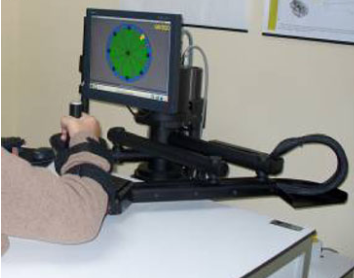
\includegraphics[width=2.5in]{InMotion2.png}
% where an .eps filename suffix will be assumed under latex, 
% and a .pdf suffix will be assumed for pdflatex; or what has been declared
% via \DeclareGraphicsExtensions.
\caption{InMotion2, showing the virtual environment the patient interacts with \cite{QuantativeRobot}}
\label{InMotion2_fig}
\end{figure}

The InMotion2 robotic rehabilitation system is an example of and end-effector system \cite{QuantativeRobot}. 
This system attaches to the patient at the forearm and wrist and allows for the motion of these 
points to be monitored in a 2D plane while the patient completes tasks shown to him on 
a screen \cite{QuantativeRobot}. Data collected from this system at the beginning and end of a course of 
rehabilitation using the system are able to show that the patient has improved at the tasks 
set by the system \cite{QuantativeRobot}.

Another end-effector system is described in \cite{VRHandFingerr}, this system is designed for 
hand and finger rehabilitation. This system is interacted with via a finger and allows you to navigate 
a point about a 3d environment on a computer, in which the patient is to complete tasks \cite{VRHandFinger}.
This system is also able to show patient improvement at the tasks after rehabilitation using the 
system \cite{VRHandFingerr}.

End-effector systems with a single attachment point give no information on the position and 
alignment of the rest of the limb. Some systems exist with two contact points (e.g. the wrist 
and the upper arm) in order to get more information but this is still limited \cite{AdvancesPush}.

\subsection{Exoskeleton}
Exoskeletal systems are systems that are built around shape and degrees of freedom of the limb \cite{AdvancesPush}. 
They allow much more information to be gathered about the limb as they allow for more sensors to be 
placed and more degrees of freedom to be monitored and controlled \cite{AdvancesPush}. It is, however, harder to 
provide support to the limb through a pure exoskeletal system, for this reason the systems are often 
hybrids; with one end of the exoskeleton attached to and end-effector system \cite{AdvancesPush}.

One such hybrid system is the ARMin rehabilitation robot which has an end-effector system for the 
shoulder attached to an exoskeleton for the elbow and the forearm \cite{ADLVE, ARMin}. The system has 4 active 
degrees of freedom and 2 passive with which to measure and guide the position and movement of 
the patient's arm \cite{ARMin}. The ARMin system is also highly adjustable at many points in its structure 
so that it can be changed to fit patients of different sizes \cite{ARMin}.

The ARMin system is also and example of a system that uses interactive games in order to increase 
patient's motivation and compliance \cite{ADLVE,ARMin}. The ARMin system was piloted on healthy subjects and 
the results of a questionnaire following this provide evidence for incorporating games increasing 
motivation \cite{ARMin}.

Another exoskeletal system for the arm is the CADEN-7 \cite{CADEN}. The CADEN-7 system was built as a 
general exoskeleton not specifically aimed at rehabilitation but suitable for use as such or as either an 
assistive device, a haptic interface or a master device for teleoperation of another robot system \cite{CADEN}. 
CADEN-7 is a 7 degree of freedom system; 3 at the shoulder, 1 at the elbow and 3 at the wrist to 
match the human arm \cite{CADEN}.

\begin{figure}[!h]
\centering
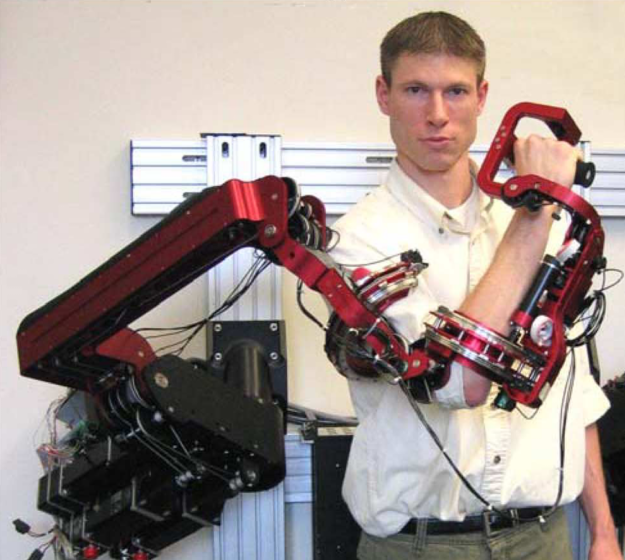
\includegraphics[width=2.5in]{CADEN7.png}
% where an .eps filename suffix will be assumed under latex, 
% and a .pdf suffix will be assumed for pdflatex; or what has been declared
% via \DeclareGraphicsExtensions.
\caption{CADEN-7 exoskeleton system \cite{CADEN}}
\label{CADEN7_fig}
\end{figure}

The name CADEN-7 comes from ``cable-actuated dexterous exoskeleton for neurorehabilitation'', 
cable actuation means the torque is transferred from motors to the part of the system to be driven 
via cables \cite{CADEN}. The advantage of this method is that they can transmit the torque over long 
distances relatively simply and without much backlash \cite{CADEN}.

Exoskeletons are possible for just the hand as well as for the entire arm. An example of such a 
system is the HEXOSYS-II \cite{HandExo}. This system has a full set of exoskeletal fingers and thumb and 
each of these can be driven to grasp and unfurl, the system also allows for the fingers to be 
spread out but this cannot be driven \cite{HandExo}.

The HEXOSYS-II has magnetic sensors by the motors in order to sense the finger position (via 
the motor position) and it also has strain gauges on the linkages between the motor and the fingers 
in order to sense the forces on the fingers \cite{HandExo}.

\section{Vision Based Systems}
\IEEEPARstart{C}{ameras} and computing power is getting cheaper all the time and are therefore 
more available. This increase in available computing power allows complex image processing to be performed 
which can be used to track a body in 2d and 3D space.

Motion capture systems such as those used for video games and film are impractical for use in 
rehabilitation as they involve a large number of high quality cameras, a clean background and 
the subject has to have markers placed on their body.

\subsection{2D Tracking Systems}
Systems based around a single video camera can only work with 2D images but can still often track 
bodies in the image and recognise gestures.

One system that tracks the motion of a hand for stroke rehabilitation purposes is described in \cite{SeriousGames}. 
This system uses a video camera and a thermal camera in order to facilitate the segmentation of the hand from the 
image against uncontrolled backgrounds \cite{SeriousGames}. The system is capable of recognising hand position 
in a 2D plane and also of distinguishing certain gestures of the hand \cite{SeriousGames}. The recognition 
of hand position and gesture is then used as the control for a pair of games designed to be appropriate to 
stroke rehabilitation \cite{SeriousGames}.

\subsection{Stereo 3D Systems}
With two cameras it is possible to capture 3D information about a scene through proper processing of the 
images. This is done by first properly aligning and calibrating the cameras and then looking at the differences 
between the two images, objects closer to the cameras will cause a greater disparity.

A system for calculating body position from the feeds of two cameras is described in \cite{StereoCamera}. This 
system takes the 'disparity map' (the differences between the two images) and uses this to first find 
the centre of gravity of this map \cite{StereoCamera}. This image is then filtered to remove both noise 
and the background \cite{StereoCamera}. With this done the system makes a decision as to whether 
you subject is self-occluded, if not then pose is calculated directly, if so then pose is calculated 
based on comparing the image to standard human body shape \cite{StereoCamera}.

\subsection{Structured Light Systems}
The Microsoft Kinect Sensor is a relatively cheap and readily available system that uses a structured 
light sensor in order to generate a depth map of a scene \cite{Kinect}. This structured light sensor 
works by projecting a grid of IR dots onto the scene and an image of these is then captured by the 
on board IR sensor, depths are then generated based on the deformation of this grid \cite{Kinect}.

\begin{figure}[!h]
\centering
\includegraphics[width=2.5in]{kinect.png}
% where an .eps filename suffix will be assumed under latex, 
% and a .pdf suffix will be assumed for pdflatex; or what has been declared
% via \DeclareGraphicsExtensions.
\caption{Kinect with sensors exposed \cite{Kinect}}
\label{kinect_fig}
\end{figure}

The Kinect Sensor comes with software for the extraction of the position of people from a scene and 
the fitting of a skeleton to them as well as gesture recognition built on top of this \cite{Kinect,kinect1}. 
This serves as an excellent starting point for use of the Kinect as a rehabilitation tool and it was 
investigated as a low cost alternative to a conventional motion capture system in \cite{kinect1} and was 
shown to be able to recognise movements with a similar level of accuracy. Another system exists that 
improves upon the gesture recognition of the Kinect allowing pose and gesture to be recognised 
simultaneously \cite{kinectGesture}.

% An example of a floating figure using the graphicx package.
% Note that \label must occur AFTER (or within) \caption.
% For figures, \caption should occur after the \includegraphics.
% Note that IEEEtran v1.7 and later has special internal code that
% is designed to preserve the operation of \label within \caption
% even when the captionsoff option is in effect. However, because
% of issues like this, it may be the safest practice to put all your
% \label just after \caption rather than within \caption{}.
%
% Reminder: the "draftcls" or "draftclsnofoot", not "draft", class
% option should be used if it is desired that the figures are to be
% displayed while in draft mode.
%
%\begin{figure}[!t]
%\centering
%\includegraphics[width=2.5in]{myfigure}
% where an .eps filename suffix will be assumed under latex, 
% and a .pdf suffix will be assumed for pdflatex; or what has been declared
% via \DeclareGraphicsExtensions.
%\caption{Simulation Results}
%\label{fig_sim}
%\end{figure}

% Note that IEEE typically puts floats only at the top, even when this
% results in a large percentage of a column being occupied by floats.


% An example of a double column floating figure using two subfigures.
% (The subfig.sty package must be loaded for this to work.)
% The subfigure \label commands are set within each subfloat command, the
% \label for the overall figure must come after \caption.
% \hfil must be used as a separator to get equal spacing.
% The subfigure.sty package works much the same way, except \subfigure is
% used instead of \subfloat.
%
%\begin{figure*}[!t]
%\centerline{\subfloat[Case I]\includegraphics[width=2.5in]{subfigcase1}%
%\label{fig_first_case}}
%\hfil
%\subfloat[Case II]{\includegraphics[width=2.5in]{subfigcase2}%
%\label{fig_second_case}}}
%\caption{Simulation results}
%\label{fig_sim}
%\end{figure*}
%
% Note that often IEEE papers with subfigures do not employ subfigure
% captions (using the optional argument to \subfloat), but instead will
% reference/describe all of them (a), (b), etc., within the main caption.


% An example of a floating table. Note that, for IEEE style tables, the 
% \caption command should come BEFORE the table. Table text will default to
% \footnotesize as IEEE normally uses this smaller font for tables.
% The \label must come after \caption as always.
%
%\begin{table}[!t]
%% increase table row spacing, adjust to taste
%\renewcommand{\arraystretch}{1.3}
% if using array.sty, it might be a good idea to tweak the value of
% \extrarowheight as needed to properly center the text within the cells
%\caption{An Example of a Table}
%\label{table_example}
%\centering
%% Some packages, such as MDW tools, offer better commands for making tables
%% than the plain LaTeX2e tabular which is used here.
%\begin{tabular}{|c||c|}
%\hline
%One & Two\\
%\hline
%Three & Four\\
%\hline
%\end{tabular}
%\end{table}


% Note that IEEE does not put floats in the very first column - or typically
% anywhere on the first page for that matter. Also, in-text middle ("here")
% positioning is not used. Most IEEE journals use top floats exclusively.
% Note that, LaTeX2e, unlike IEEE journals, places footnotes above bottom
% floats. This can be corrected via the \fnbelowfloat command of the
% stfloats package.

\section{Discussion}
\IEEEPARstart{T}{here} are a wide range of approaches to the problem of stroke rehabilitation systems, 
each has its benefits and drawbacks and it may be the case that more than one 
could be used in a patient's care.

Purely passive sensor based systems provide information on the limb they're 
monitoring but are unable to support or assist it. They are much lighter 
and less complex than actuated systems and this might give them an advantage 
in certain areas of the patient's care; for instance it might be that the 
system is compact enough that it is something that a physiotherapist could 
take with them for use in house calls.

Accelerometers are versatile sensors that can be used for inferred position and angle 
measurements depending on their arrangement. Passive sensing of angle is best done by 
potentiometer but for measuring the position of a driven joint a magnetometer can 
be used next to the motor. FSRs and QTCs are the most useful way to sense force for 
this sort of system and these are used usually in hand/ grip rehabilitation systems.

End-effector type systems are useful and fairly simple but limited, whereas 
exoskeletons are more complex systems but give more information. The main 
challenge of an exoskeleton system is to match the degrees of freedom and 
range of movement of the human arm and, in the interests of safety, not be 
able to exceed these.

End-effector and Exoskeleton systems for the whole arm tend to be very large, 
usually wall mounted, systems. This allows them to properly actuate and drive the 
complete arm throughout its range of motion. There are also end-effector and 
exoskeleton systems for the hand and fingers which are also important to 
include in the rehabilitation scheme.

Visual systems are potentially the cheapest candidate for rehabilitation systems. 
Single camera based systems are limited in the movements they can recognise as 
they can't extract 3D information whereas multiple camera systems can meaning 
that they can potentially recognise more complex movements.

The Kinect sensor enables low-cost motion tracking and provides an environment 
for further experimentation providing a huge amount of potential for 
rehabilitation systems

\section{Conclusion}
\IEEEPARstart{A}{stroke} can affect a person in a multitude of ways including fully or 
partially paralysing them down one or both sides. The damage caused can however be 
mitigated by rehabilitation due to the brain's plasticity.

Robotic sensor systems are shown to have potential as useful tools to the 
physiotherapist and for engaging the patient with their rehabilitation.

There are two main areas where robotic/sensor rehabilitation systems are appropriate; 
in the hospital for the acute and rehabilitation stages of care, these can big bulky 
systems, and in the home for the rehabilitation and community stages of care, these 
have to be smaller and much cheaper systems.

The big end-effector and full arm exoskeleton systems are more suited to the hospital 
where they can be used as advanced tools for the physiotherapist, providing detailed 
feedback on the patient's movements.

Systems based around a few sensors placed on the arm or on visual sensors are more 
suitable for home use, particularly when used as a haptic interface and linked to 
a game designed to encourage the patient to do appropriate actions for their 
rehabilitation. 

Linking the system to a game is a popular way to increase the patient's motivation and 
thereby increase the effectiveness of the rehabilitation program due to increased 
repetition. Almost all the systems developed with rehabilitation in mind linked 
their system to some form of game or simulation of activities of daily life.




% if have a single appendix:
%\appendix[Proof of the Zonklar Equations]
% or
%\appendix  % for no appendix heading
% do not use \section anymore after \appendix, only \section*
% is possibly needed

% use appendices with more than one appendix
% then use \section to start each appendix
% you must declare a \section before using any
% \subsection or using \label (\appendices by itself
% starts a section numbered zero.)
%


%\appendices
%\section{Hopefully won't have any of these}
%Appendix one text goes here.

% you can choose not to have a title for an appendix
% if you want by leaving the argument blank
%\section{}
%Appendix two text goes here.


% use section* for acknowledgement
%\section*{Acknowledgment}


%The authors would like to thank...


% Can use something like this to put references on a page
% by themselves when using endfloat and the captionsoff option.
\ifCLASSOPTIONcaptionsoff
  \newpage
\fi



% trigger a \newpage just before the given reference
% number - used to balance the columns on the last page
% adjust value as needed - may need to be readjusted if
% the document is modified later
%\IEEEtriggeratref{8}
% The "triggered" command can be changed if desired:
%\IEEEtriggercmd{\enlargethispage{-5in}}

% references section

% can use a bibliography generated by BibTeX as a .bbl file
% BibTeX documentation can be easily obtained at:
% http://www.ctan.org/tex-archive/biblio/bibtex/contrib/doc/
% The IEEEtran BibTeX style support page is at:
% http://www.michaelshell.org/tex/ieeetran/bibtex/
%\bibliographystyle{IEEEtran}
% argument is your BibTeX string definitions and bibliography database(s)
%\bibliography{library}
%
% <OR> manually copy in the resultant .bbl file
% set second argument of \begin to the number of references
% (used to reserve space for the reference number labels box)

\begin{thebibliography}{1} 
  
\bibitem{NSA} National STROKE Association. (2012, April 14). \emph{Effects of Stroke} [Online]. Available: \url{http://www.stroke.org/site/PageServer?pagename=EFFECT}

\bibitem{TheBrain} J. Caswell. (2012, April 11). \emph{A Tour of the Brain} [Online]. Available: \url{http://www.strokeassociation.org/STROKEORG/AboutStroke/EffectsofStroke/ATouroftheBrain/A-Tour-of-the-Brain_UCM_310943_Article.jsp}

\bibitem{Physio} physiotherapy-treatment.com (2012, April 5). \emph{stroke physical therapy} [Online]. Available: \url{http://www.physiotherapy-treatment.com/stroke-physical-therapy.html}

\bibitem{fuglmeyer} F.-meyer Ar, L. Jaasko, I. Leyman, S. Olsson, and S. S. The, “FUGL-MEYER ASSESSMENT UPPER EXTREMITY ( FMA-UE ) Assessment of sensorimotor function”, 2, pp. 1-3, 2010.

\bibitem{VRHandFingerr} O. a. Daud, R. Oboe, M. Agostini, and A. Turolla, “Performance evaluation of a VR-based hand and finger rehabilitation program,” 2011 IEEE International Symposium on Industrial Electronics, pp. 934-939, Jun. 2011.

\bibitem{flexiSensor} S. Dohta, T. Akagi, and H. Kuno, “Development of string-type flexible displacement sensor to measure the movement of robot and human body,” International journal of Mechatronics and Machine Vision in Practice, pp. 2-4, 2010.

\bibitem{ACangle} F. Ghassemi, S. Tafazoli, and P. Lawrence, “Design and Calibration of an Integration-Free Accelerometer-Based Joint-Angle Sensor,” IEEE Transactions on Instrumentation and Measurement, vol. 57, no. 1, pp. 150-159, 2008.

\bibitem{ACfeasable} D. Giansanti and V. Macellari, “Is it feasible to reconstruct body segment 3-D position and orientation using accelerometric data?,” IEEE Transactions on Biomedical Engineering, vol. 50, no. 4, pp. 476-483, 2003.

\bibitem{ADLVE} M. Guidali, A. Duschau-Wicke, S. Broggi, V. Klamroth-Marganska, T. Nef, and R. Riener, “A robotic system to train activities of daily living in a virtual environment.,” Medical \& biological engineering \& computing, vol. 49, no. 10, pp. 1213-23, Oct. 2011.

\bibitem{ACSVM} L. Guo and L. Yu, “Upper limb motion recognition for unsupervised stroke rehabilitation based on Support Vector Machine,” Bioelectronics and Bioinformatics (ISBB), 2011.

\bibitem{FSR} A. Hollinger, “Evaluation of commercial force-sensing resistors,” Unpublished report, pp. 1-4, 2006.

\bibitem{QTCs} Peratech. (2012, May 7). \emph{QTC Material} [Online]. Available: \url{http://www.peratech.com/qtcmaterial.php}

\bibitem{Interlink} Interlink Electronics Inc. (2011). \emph{Force Sensorsl} [Online]. Available: \url{http://www.interlinkelectronics.com/catalog/Force-Sensors}

\bibitem{HandExo} J. Iqbal, N. G. Tsagarakis, and D. G. Caldwell, “A multi-DOF robotic exoskeleton interface for hand motion assistance,” 2011 Annual International Conference of the IEEE Engineering in Medicine and Biology Society, pp. 1575-1578, Aug. 2011.

\bibitem{StereoCamera} S. Jun, J. Park, C. Park, and I. Jung, “Morphological approach of stereo camera based human motion capture system,” International Conference on Control, Automation and Systems, 2007., pp. 2238-2241, 2007.

\bibitem{AdvancesPush} R. C. V. Loureiro, W. S. Harwin, K. Nagai, and M. Johnson, “Advances in upper limb stroke rehabilitation: a technology push.,” Medical \& biological engineering \& computing, vol. 49, no. 10, pp. 1103-18, Oct. 2011.

\bibitem{lowCostACs} M. Mui, “Development and characterizations of low cost accelerometers,” Electronic Materials and Packaging,, 2006.

\bibitem{ARMin} T. Nef, M. Mihelj, and G. Colombo, “ARMin-robot for rehabilitation of the upper extremities,” Robotics and Automation,, no. May, pp. 3152-3157, 2006.

\bibitem{PLEMO} T. Ozawa et al., “Initial clinical tests for assessment models of synergy movements of stroke patients using PLEMO system with sensor grip device,” 2009 IEEE International Conference on Rehabilitation Robotics, pp. 873-878, Jun. 2009.

\bibitem{CADEN} J. Perry and J. Rosen, “Upper-limb powered exoskeleton design,” Mechatronics, IEEE/ASME, vol. 12, no. 4, pp. 408-417, 2007.

\bibitem{QuantativeRobot} L. Zollo, L. Rossini, M. Bravi, G. Magrone, S. Sterzi, and E. Guglielmelli, “Quantitative evaluation of upper-limb motor control in robot-aided rehabilitation.,” Medical \& biological engineering \& computing, vol. 49, no. 10, pp. 1131-44, Oct. 2011.

\bibitem{SeriousGames} L. Evett et al., “Dual camera motion capture for serious games in stroke rehabilitation,” 2011 IEEE 1st International Conference on Serious Games and Applications for Health (SeGAH), pp. 1-4, Nov. 2011.

\bibitem{kinect1} C. Schonauer, T. Pintaric, and H. Kaufmann, “Chronic pain rehabilitation with a serious game using multimodal input,” International Conference on Virtual Rehabilitation, 2011.

\bibitem{Kinect} W. Zeng and Z. Zhang, “Multimedia at Work Microsoft Kinect Sensor and Its Effect,” pp. 4-10, 2012.

\bibitem{kinectGesture} A. Bigdelou, T. Benz, L. Schwarz, and N. Navab, “Simultaneous categorical and spatio-temporal 3D gestures using Kinect,” 2012 IEEE Symposium on 3D User Interfaces (3DUI), pp. 53-60, Mar. 2012.

\end{thebibliography}

% biography section
% 
% If you have an EPS/PDF photo (graphicx package needed) extra braces are
% needed around the contents of the optional argument to biography to prevent
% the LaTeX parser from getting confused when it sees the complicated
% \includegraphics command within an optional argument. (You could create
% your own custom macro containing the \includegraphics command to make things
% simpler here.)
%\begin{biography}[{\includegraphics[width=1in,height=1.25in,clip,keepaspectratio]{mshell}}]{Michael Shell}
% or if you just want to reserve a space for a photo:

%\begin{IEEEbiography}{Michael Shell}
%Biography text here.
%\end{IEEEbiography}

% if you will not have a photo at all:

% insert where needed to balance the two columns on the last page with
% biographies
%\newpage


% You can push biographies down or up by placing
% a \vfill before or after them. The appropriate
% use of \vfill depends on what kind of text is
% on the last page and whether or not the columns
% are being equalized.

%\vfill

% Can be used to pull up biographies so that the bottom of the last one
% is flush with the other column.
%\enlargethispage{-5in}



% that's all folks
\end{document}


